\section{Aggregation and Deaggregation Strategies}
\label{sec:agdag}

One of the primary drawbacks of Algorithm~\ref{alg:algoHybrid} is in handling the discrete transitions. 
%
Suppose that in a given location, the number of stars that overlap with the guard of a discrete transition (line~\ref{ln:guardIntersection} in Algorithm~\ref{alg:algoHybrid}) is $m$.
%
As a result, the number of stars in the $queueStars$ will become $O(m^2)$ after 2 discrete. After $t$ number of discrete transitions, the number of states in $queueStars$ grows to $O(m^t)$.
%
To avoid the exponential blow up of the number of sets in $queueStars$, reachable set computation tools often use aggregation.

In aggregation, the set of all stars in $queueStars$ that are making a discrete transition to the same mode are collected together. 
%
Say, these states are $S_1, S_2, \ldots, S_m$.
%
Then, an overapproximation of these $S'$ is computed such that $S_1 \cup S_2 \cup S_3 \ldots \cup S_m \subseteq S'$. 
%
Instead of computing the reachable set for each of $S_1, S_2, \ldots, S_m$, the reachable set of $S'$ is computed in the future modes.

There are two main drawbacks of this aggregation mechanism. 
%
First, the collection of sets $S_1, S_2, \ldots, S_m$ is often a non-convex set. 
%
Whereas the representation used for computing reachable set is for convex sets. 
%
Therefore, this overapproximation of a non-convex set by a convex set is very conservative.
%
More worryingly, the reachable set of $S'$ will trigger additional discrete transitions that would not happen while computing the reachable sets using $S_1, S_2, \ldots, S_m$.
%
Such discrete transitions are artifacts of the conservative overapproximation during the aggregation process.

\begin{figure}[t]
\centerline{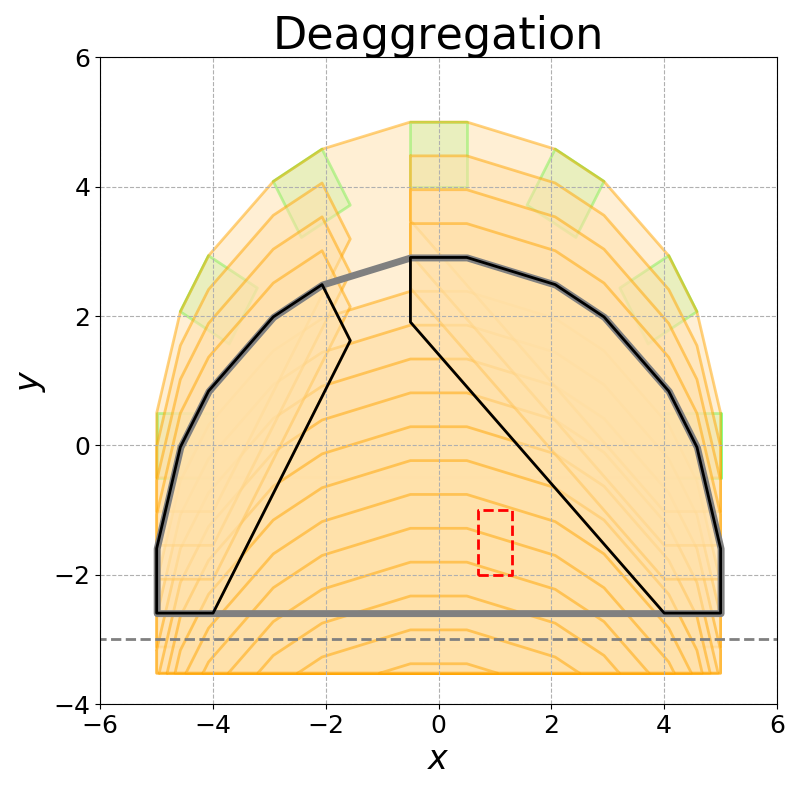
\includegraphics[width=0.8\columnwidth]{images/deagg.png}}
\caption{The deaggregation process is shown for a two-mode system. Upon reaching an error mode (red dotted region), the fully aggregated set of states (gray large region), is split in half (two black regions), which no longer contain error states. A video of the complete computation is available online at \url{https://youtu.be/SDzGKDBq5tM}.}
\label{fig:deagg}
\end{figure}

To overcome the above mentioned challenges, we develop new aggregation and deaggregation techniques. Our technique works the following way. 
First, while handling discrete transitions, we perform aggregation for all the sets in the $queueStars$ that go to the same mode. 
%
The resultant star is tagged as an \textsf{aggregate} and the reachable set computation continues where the sets are tagged as \textsf{aggregate}. 
%
This way of computing the reachable set will result in a conservative overapproximation.
%
If one of the sets in the computation overlaps with the unsafe set $U$, we check if the set is tagged as \textsf{aggregate}.
%
If so, then we go to the initial set in the location that caused this overapproximation and deaggregate this 
